% !TEX program = xelatex (Tectonic)
\documentclass[11pt,a4paper]{article}

\usepackage{fontspec}
\usepackage[french]{babel}
\usepackage[a4paper,margin=2.3cm]{geometry}
\usepackage{xcolor}
\usepackage{booktabs}
\usepackage{graphicx}
\usepackage{titlesec}
\usepackage{enumitem}
\usepackage[hidelinks]{hyperref}

%======================= Couleurs (mêmes que tp-scraping / tp-dataanalysis) =======================
\definecolor{primary}{HTML}{1F4E79}
\definecolor{accent}{HTML}{C0392B}
\definecolor{soft}{HTML}{5B7A9A}
\definecolor{lightbg}{HTML}{EEF3F8}

\titleformat{\section}{\Large\bfseries\color{primary}}{\thesection.}{0.5em}{}
\titleformat{\subsection}{\large\bfseries\color{soft}}{\thesubsection}{0.5em}{}

\newcommand{\ok}{\textcolor{primary}{\bfseries Conforme}}
\newcommand{\siteurl}{\href{https://academic.hermann-agossou.com}{\texttt{academic.hermann-agossou.com}}}

\begin{document}

%======================= En-tête =======================
\begin{center}
  {\color{soft}Module Digitalisation \textbullet\ Pr.\ Omar Zahour}\\[1.2em]
  {\color{primary}\bfseries\LARGE Projet de module — Site personnel académique}\\[0.5em]
  {\color{soft}\large \siteurl}\\[1.2em]
  Hermann Agossou\\[0.3em]
  {\color{soft}\small Juillet 2026}
\end{center}

\vspace{0.8em}

%======================= Objectif =======================
\section{Objectif et choix technique}

Le cahier des charges demande un site personnel servant de vitrine académique :
au moins six pages (Accueil, CV, Publications, Communications \& Attestations,
Cours \& TPs, Parcours \& Contact), dix références Zotero ou plus, cinq
attestations téléchargeables, un formulaire de contact fonctionnel et une page
Mentions légales / RGPD.

Le site est publié à l'adresse \siteurl. Plutôt que Google Sites, il est
construit avec le générateur de sites statiques
\href{https://astro.build}{Astro}, versionné sur GitHub (dépôt
\href{https://github.com/Hermann-web/academic}{\texttt{Hermann-web/academic}})
et déployé automatiquement sur GitHub Pages derrière un sous-domaine
personnalisé. Ce choix, assumé, va dans le sens des objectifs du module : le
contenu est plus durable (code source versionné, hébergement gratuit et
pérenne), plus facilement actualisable (chaque mise à jour est un simple
\texttt{git push}, le déploiement est automatique) et l'identité numérique est
renforcée par un domaine propre. Tous les livrables demandés (export Zotero,
CV~PDF, attestations, formulaire Google Forms, wireframe draw.io) restent
identiques à ceux attendus.

\section{Conformité au cahier des charges}

\begin{center}
  \renewcommand{\arraystretch}{1.35}
  \small
  \begin{tabular}{p{5.6cm}p{6.6cm}l}
    \toprule
    \textbf{Exigence} & \textbf{Réalisation} & \textbf{Statut} \\
    \midrule
    Site structuré en 6 pages minimum & 7 pages publiées (les six demandées +
      Mentions légales \& RGPD) & \ok \\
    Au moins 10 références Zotero & Collection « COURSDIGIT » de 14 références,
      affichées sur la page Publications ; export \texttt{.bib} téléchargeable
      depuis le site & \ok \\
    5 attestations téléchargeables & 9 attestations PDF (enseignement,
      encadrement, organisation, participation) & \ok \\
    Formulaire de contact fonctionnel & Google Forms intégré à la page
      Parcours \& Contact
      (\href{https://forms.gle/J4Ha9enVPYWr71S49}{\texttt{forms.gle/J4Ha9enVPYWr71S49}}) & \ok \\
    CV au format PDF intégré & Visionneuse PDF intégrée + bouton de
      téléchargement ; CV généré depuis LaTeX & \ok \\
    3 supports de cours hébergés & 5 supports PDF hébergés sur le site
      (Coding Week : cours Git, TP GitHub, sujet de projet ; Programmation :
      TP~1, sujet de projet) & \ok \\
    Biographie, parcours, profils & Chronologie détaillée + liens LinkedIn,
      ResearchGate, GitHub, PyPI & \ok \\
    Mentions légales \& RGPD & Page dédiée : données personnelles, absence de
      traceurs, licences (CC~BY~4.0), droits des visiteurs & \ok \\
    Wireframe draw.io & Fichier \texttt{docs/wireframe.drawio} dans le dépôt
      (arborescence reprise en figure~\ref{fig:arbo}) & \ok \\
    Responsive, navigation intuitive & Menu commun à toutes les pages, mise en
      page adaptative testée mobile/desktop (figure~\ref{fig:mobile}) & \ok \\
    \bottomrule
  \end{tabular}
\end{center}

\section{Arborescence du site}

\begin{figure}[htbp]
  \centering
  \renewcommand{\arraystretch}{1.3}
  \small
  \begin{tabular}{ll}
    \toprule
    \textbf{Page} & \textbf{URL} \\
    \midrule
    Accueil & \texttt{/} \\
    CV & \texttt{/cv} \\
    Publications & \texttt{/publications} \\
    Communications \& Attestations & \texttt{/communications-attestations} \\
    Cours \& TPs & \texttt{/cours-tps} \\
    Parcours \& Contact & \texttt{/parcours-contact} \\
    Mentions légales \& RGPD & \texttt{/mentions-legales} \\
    \bottomrule
  \end{tabular}
  \caption{Arborescence publiée (chaque URL est relative à \siteurl).}
  \label{fig:arbo}
\end{figure}

\section{Captures d'écran}

Les captures suivantes proviennent du site en ligne (\siteurl),
prises le 19 juillet 2026.

\begin{figure}[htbp]
  \centering
  \fbox{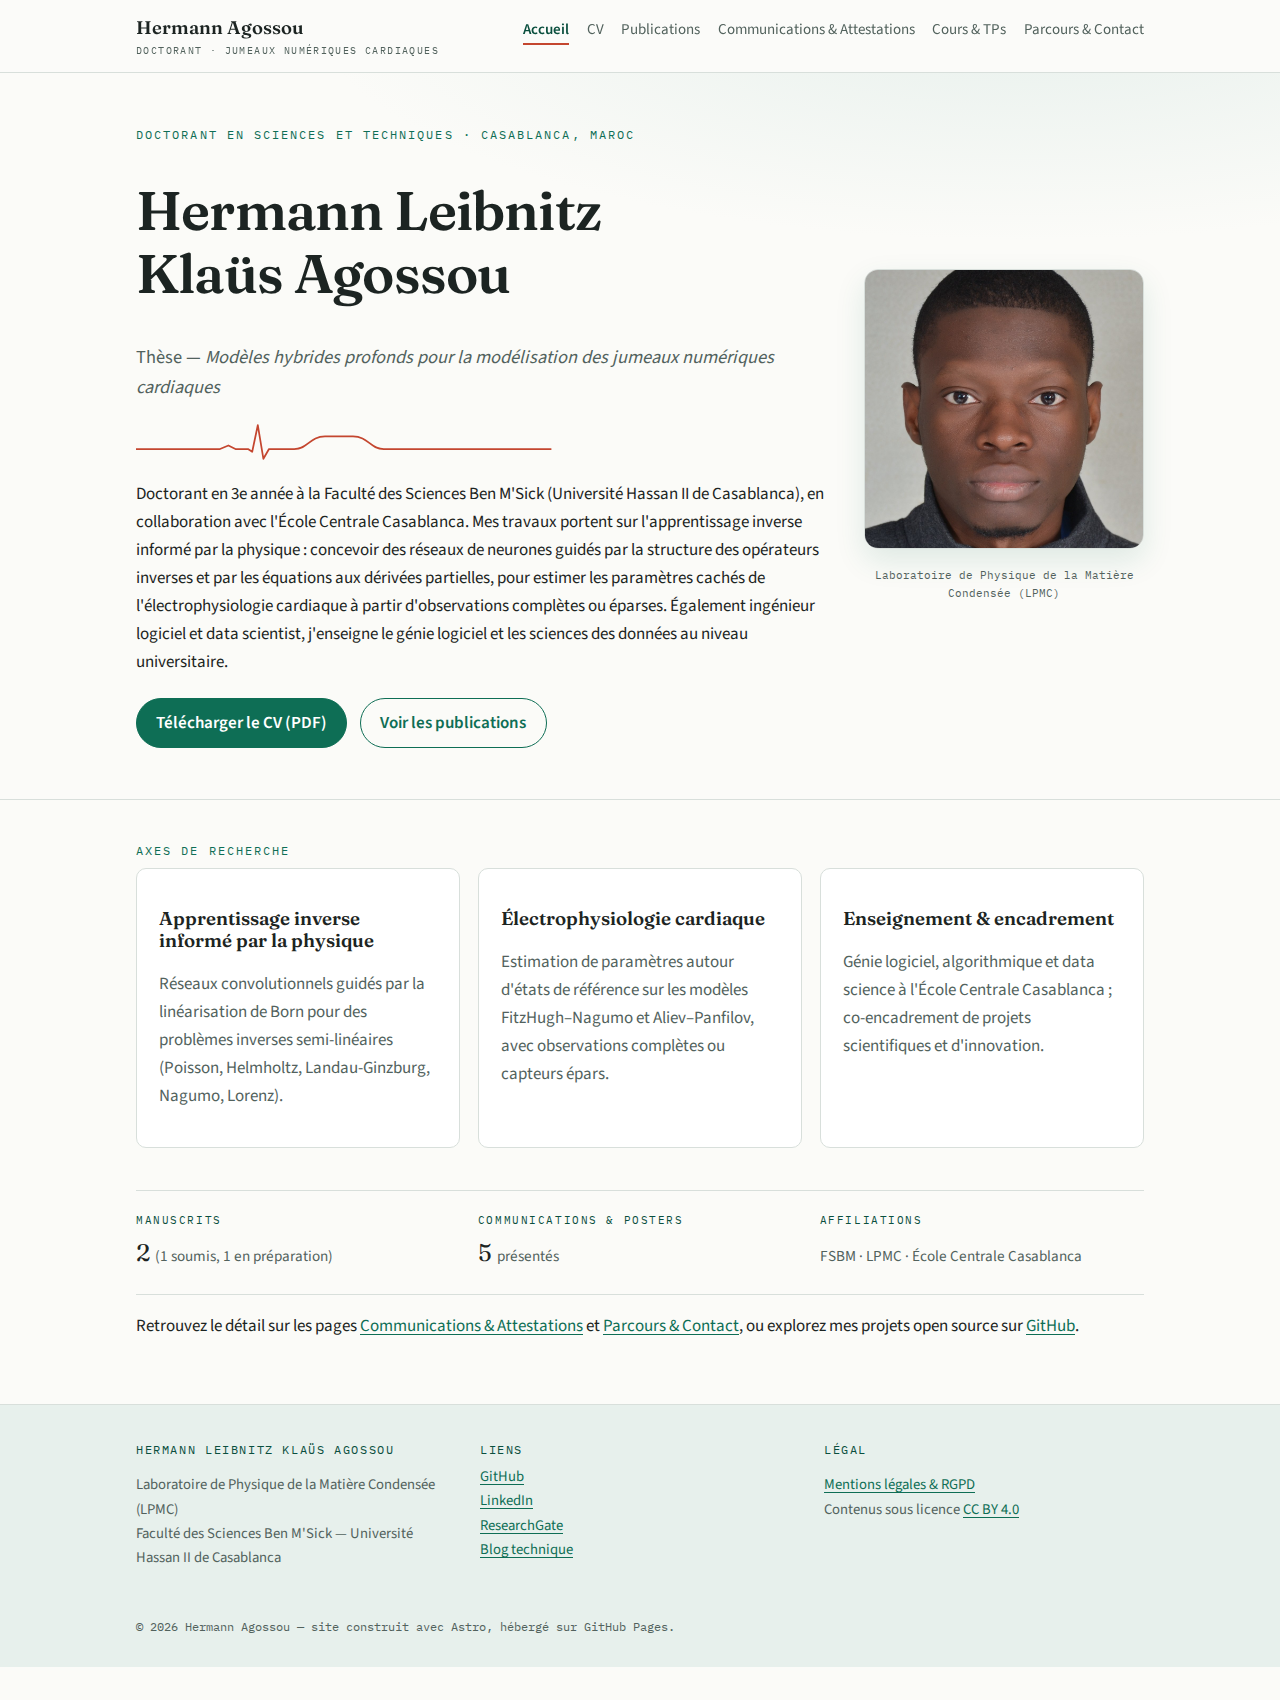
\includegraphics[width=0.96\linewidth]{assets/accueil.png}}
  \caption{Accueil : photo, nom, discipline, résumé du profil, menu de
    navigation et axes de recherche.}
  \label{fig:accueil}
\end{figure}

\begin{figure}[htbp]
  \centering
  \fbox{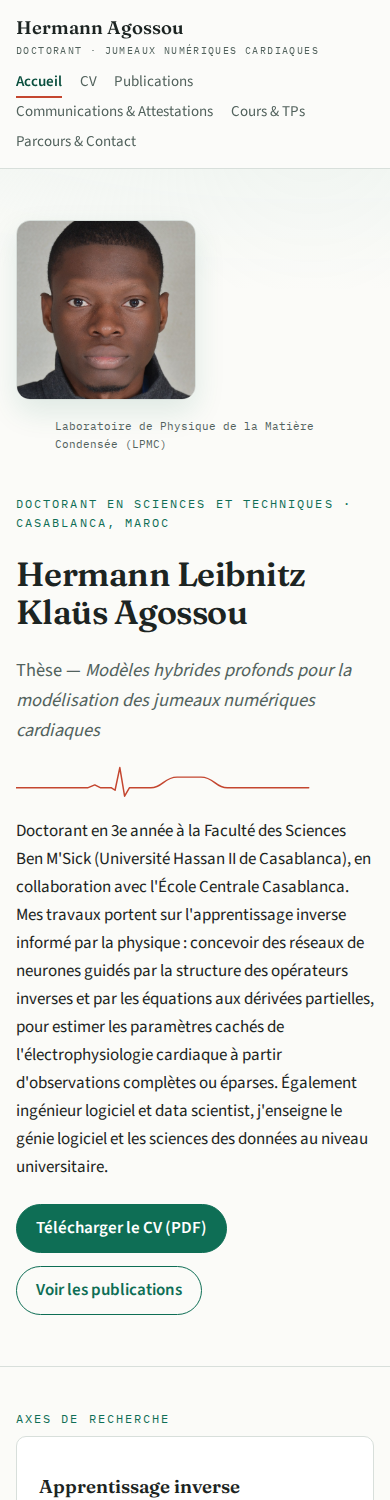
\includegraphics[width=0.30\linewidth]{assets/accueil-mobile.png}}
  \caption{Accueil sur mobile (390~px de large) : la mise en page s'adapte,
    critère « ergonomie \& design ».}
  \label{fig:mobile}
\end{figure}

\begin{figure}[htbp]
  \centering
  \fbox{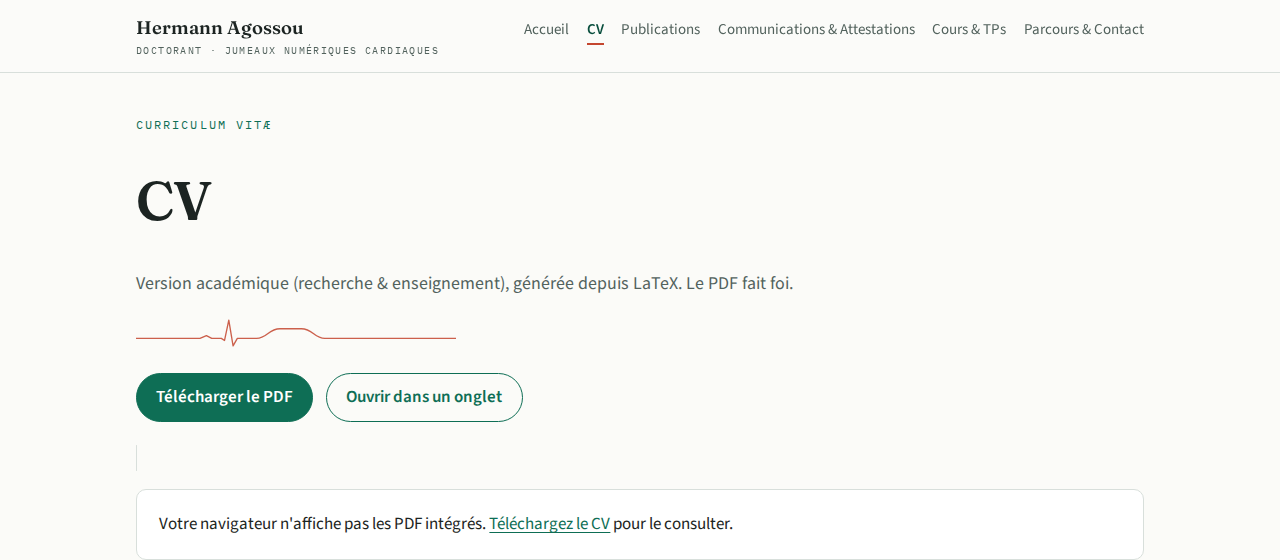
\includegraphics[width=0.96\linewidth]{assets/cv.png}}\\[0.6em]
  \fbox{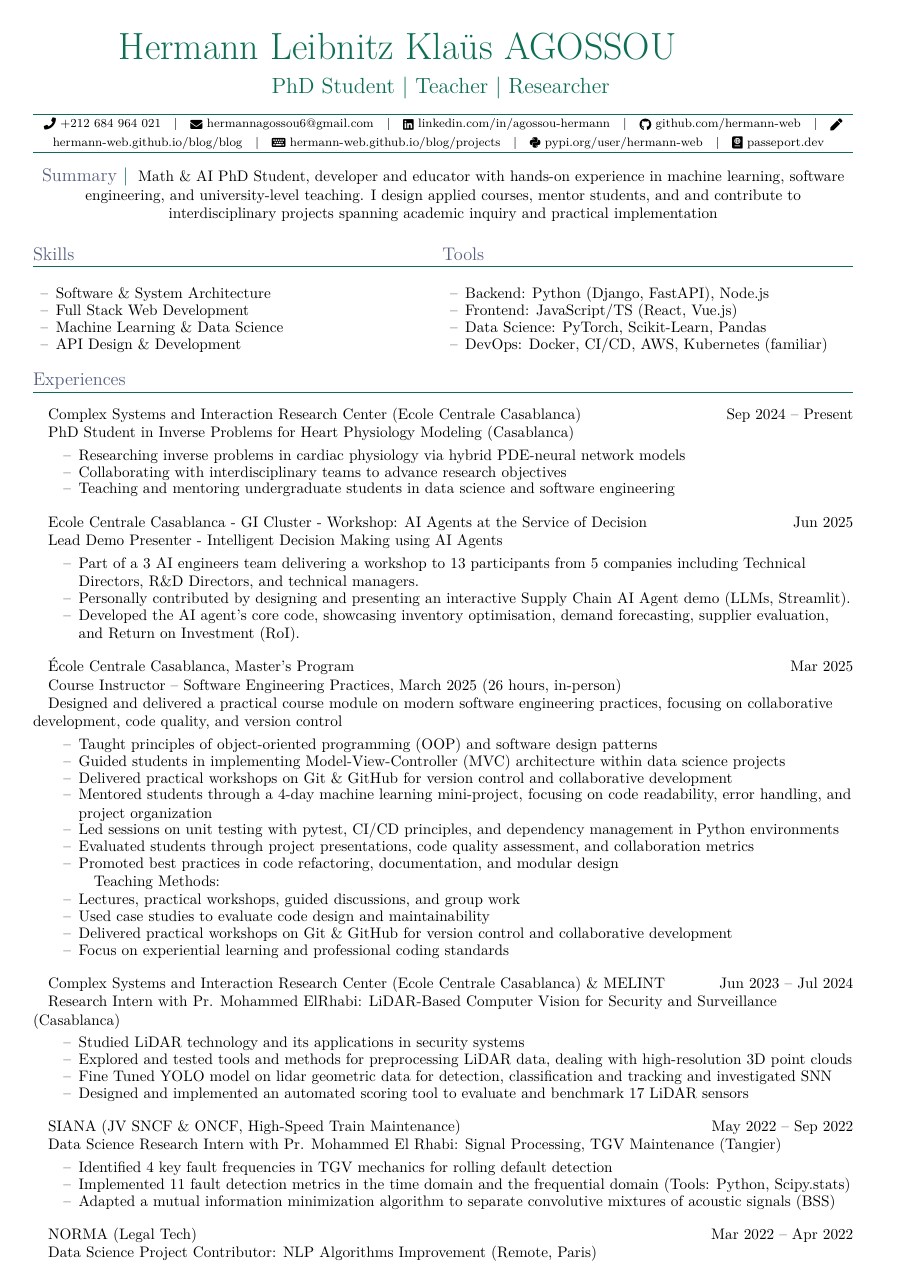
\includegraphics[width=0.58\linewidth]{assets/cv-pdf-page1.png}}
  \caption{Page CV : boutons de téléchargement et visionneuse intégrée (haut) ;
    première page du fichier \texttt{hermann-agossou-cv.pdf} tel que servi par
    le site (bas). L'outil de capture utilisé n'affiche pas les PDF intégrés,
    contrairement aux navigateurs classiques.}
  \label{fig:cv}
\end{figure}

\begin{figure}[htbp]
  \centering
  \fbox{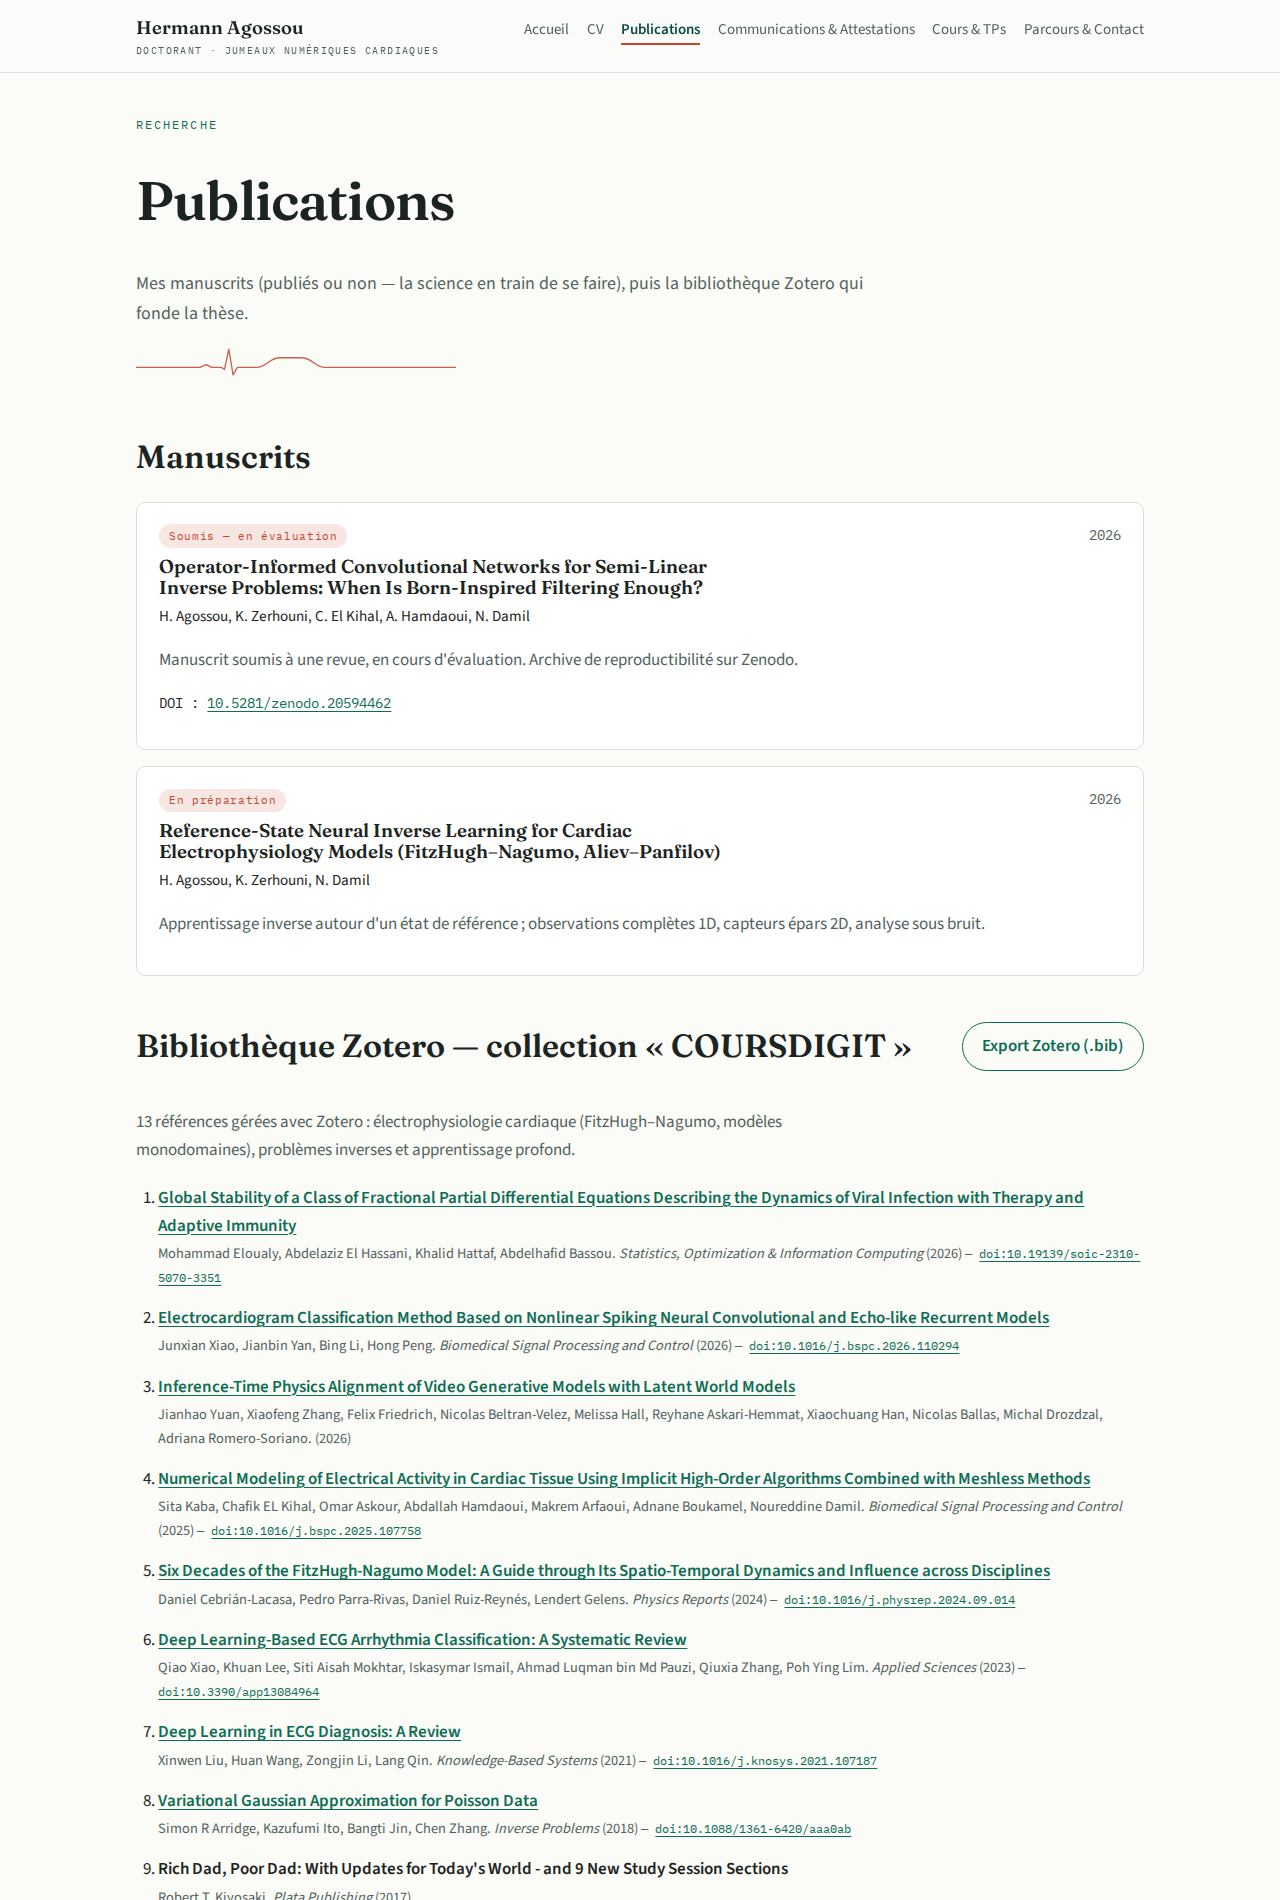
\includegraphics[width=0.96\linewidth]{assets/publications.png}}
  \caption{Publications : manuscrits personnels (soumis / en préparation, DOI
    Zenodo) puis bibliothèque Zotero avec bouton « Export Zotero (.bib) ».}
  \label{fig:publications}
\end{figure}

\begin{figure}[htbp]
  \centering
  \fbox{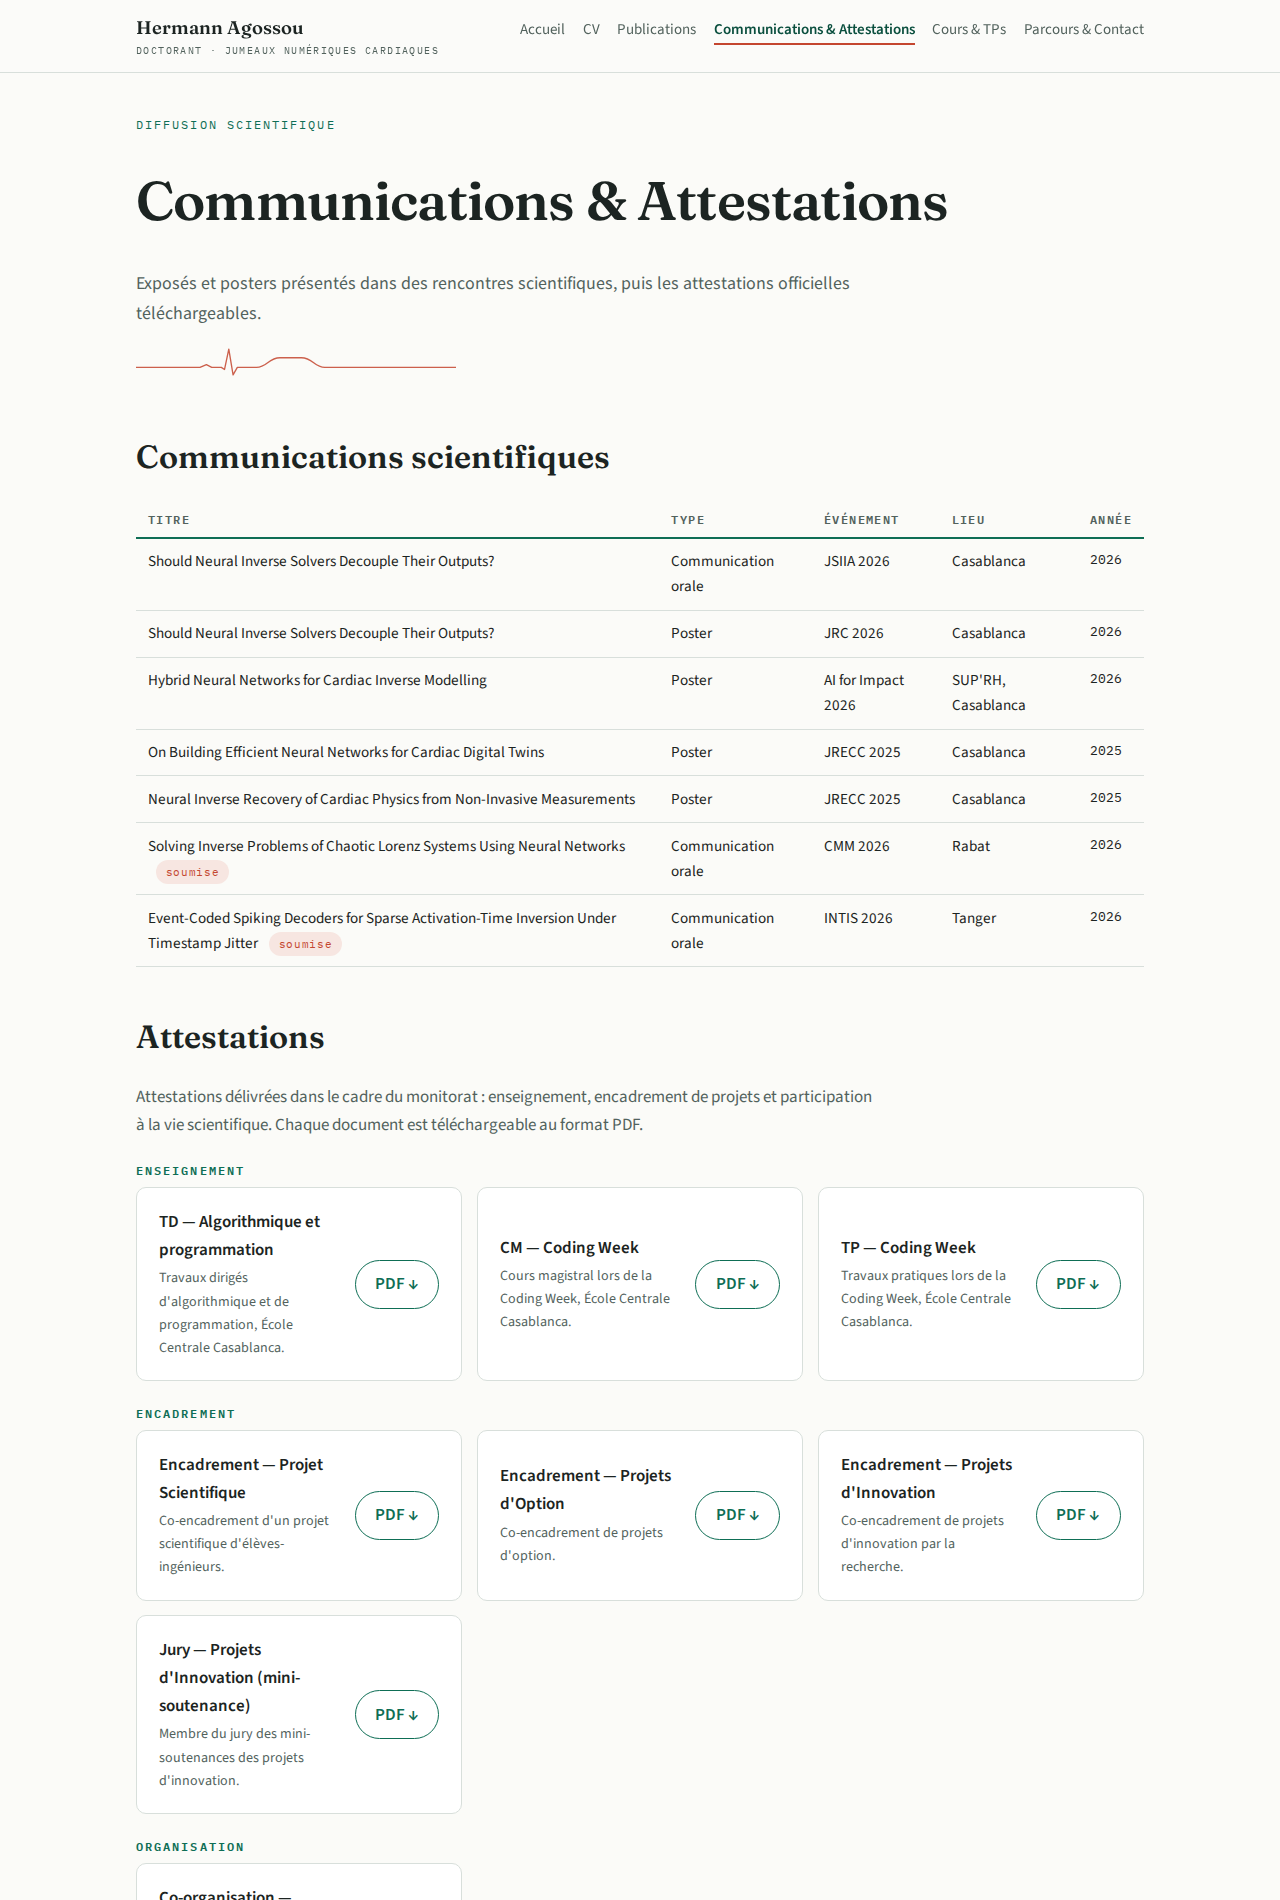
\includegraphics[width=0.96\linewidth]{assets/communications.png}}
  \caption{Communications \& Attestations : tableau des communications (titre,
    type, événement, lieu, année) et attestations téléchargeables groupées par
    catégorie.}
  \label{fig:communications}
\end{figure}

\begin{figure}[htbp]
  \centering
  \fbox{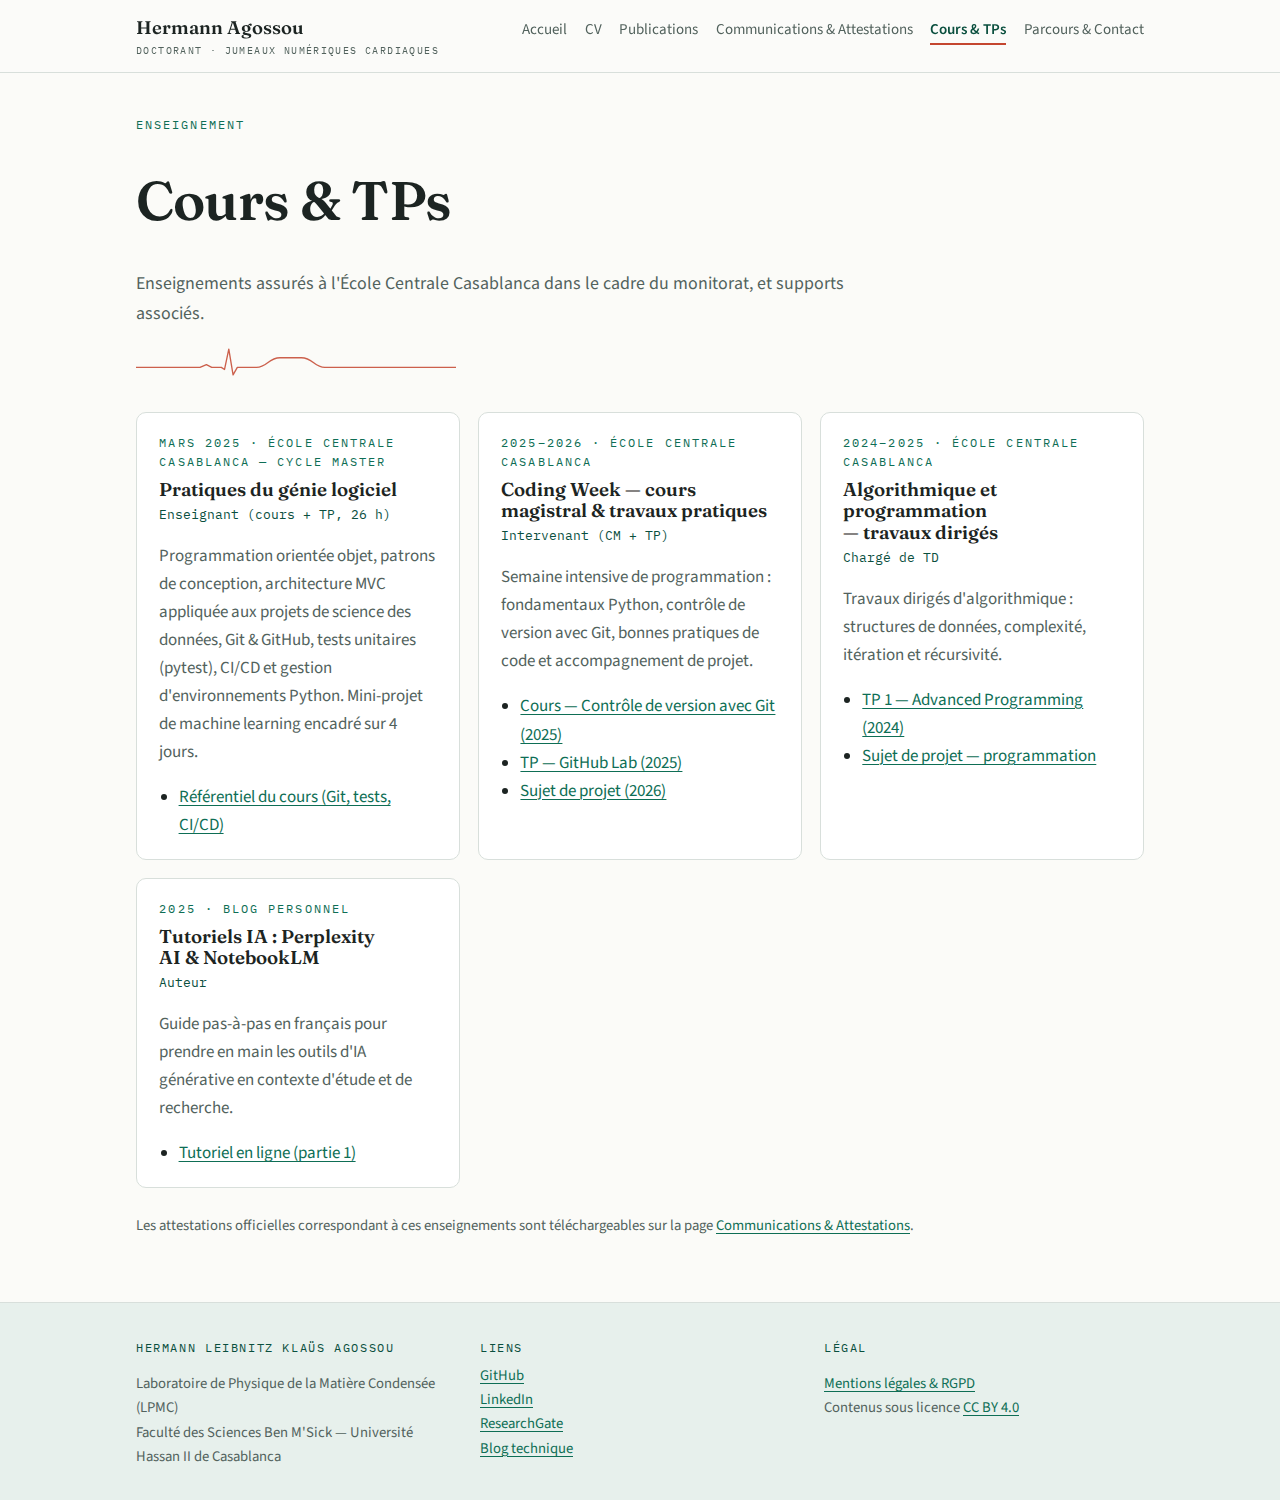
\includegraphics[width=0.96\linewidth]{assets/cours.png}}
  \caption{Cours \& TPs : enseignements assurés et supports PDF hébergés sur le
    site.}
  \label{fig:cours}
\end{figure}

\begin{figure}[htbp]
  \centering
  \fbox{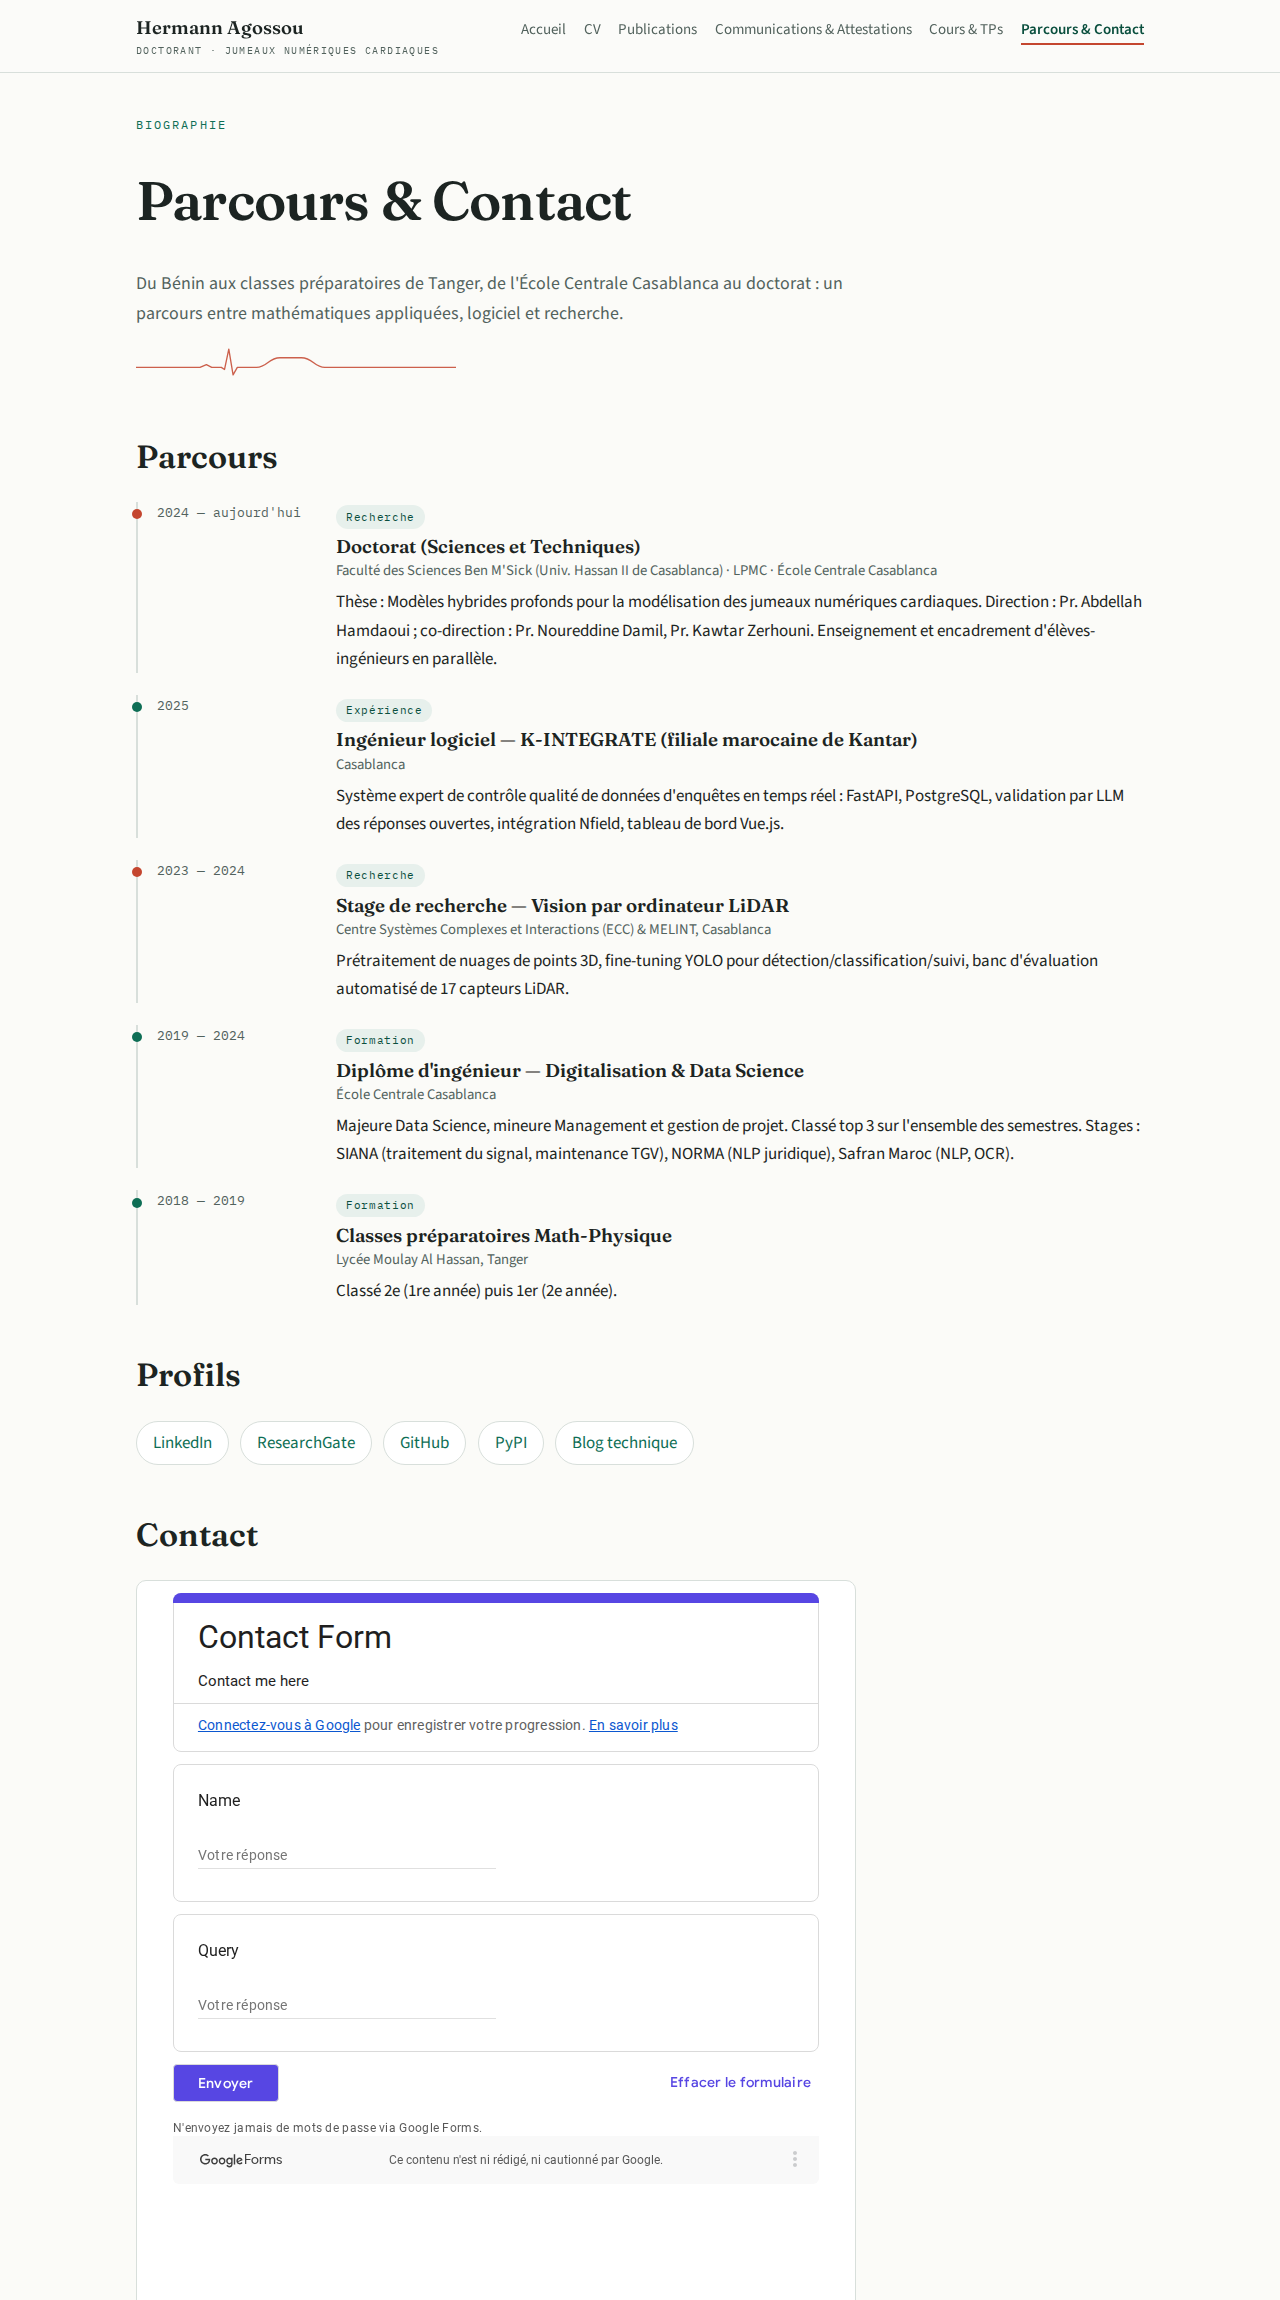
\includegraphics[width=0.96\linewidth]{assets/contact.png}}
  \caption{Parcours \& Contact : chronologie du parcours, profils
    (LinkedIn, ResearchGate, GitHub, PyPI) et formulaire Google Forms intégré et
    fonctionnel.}
  \label{fig:contact}
\end{figure}

\begin{figure}[htbp]
  \centering
  \fbox{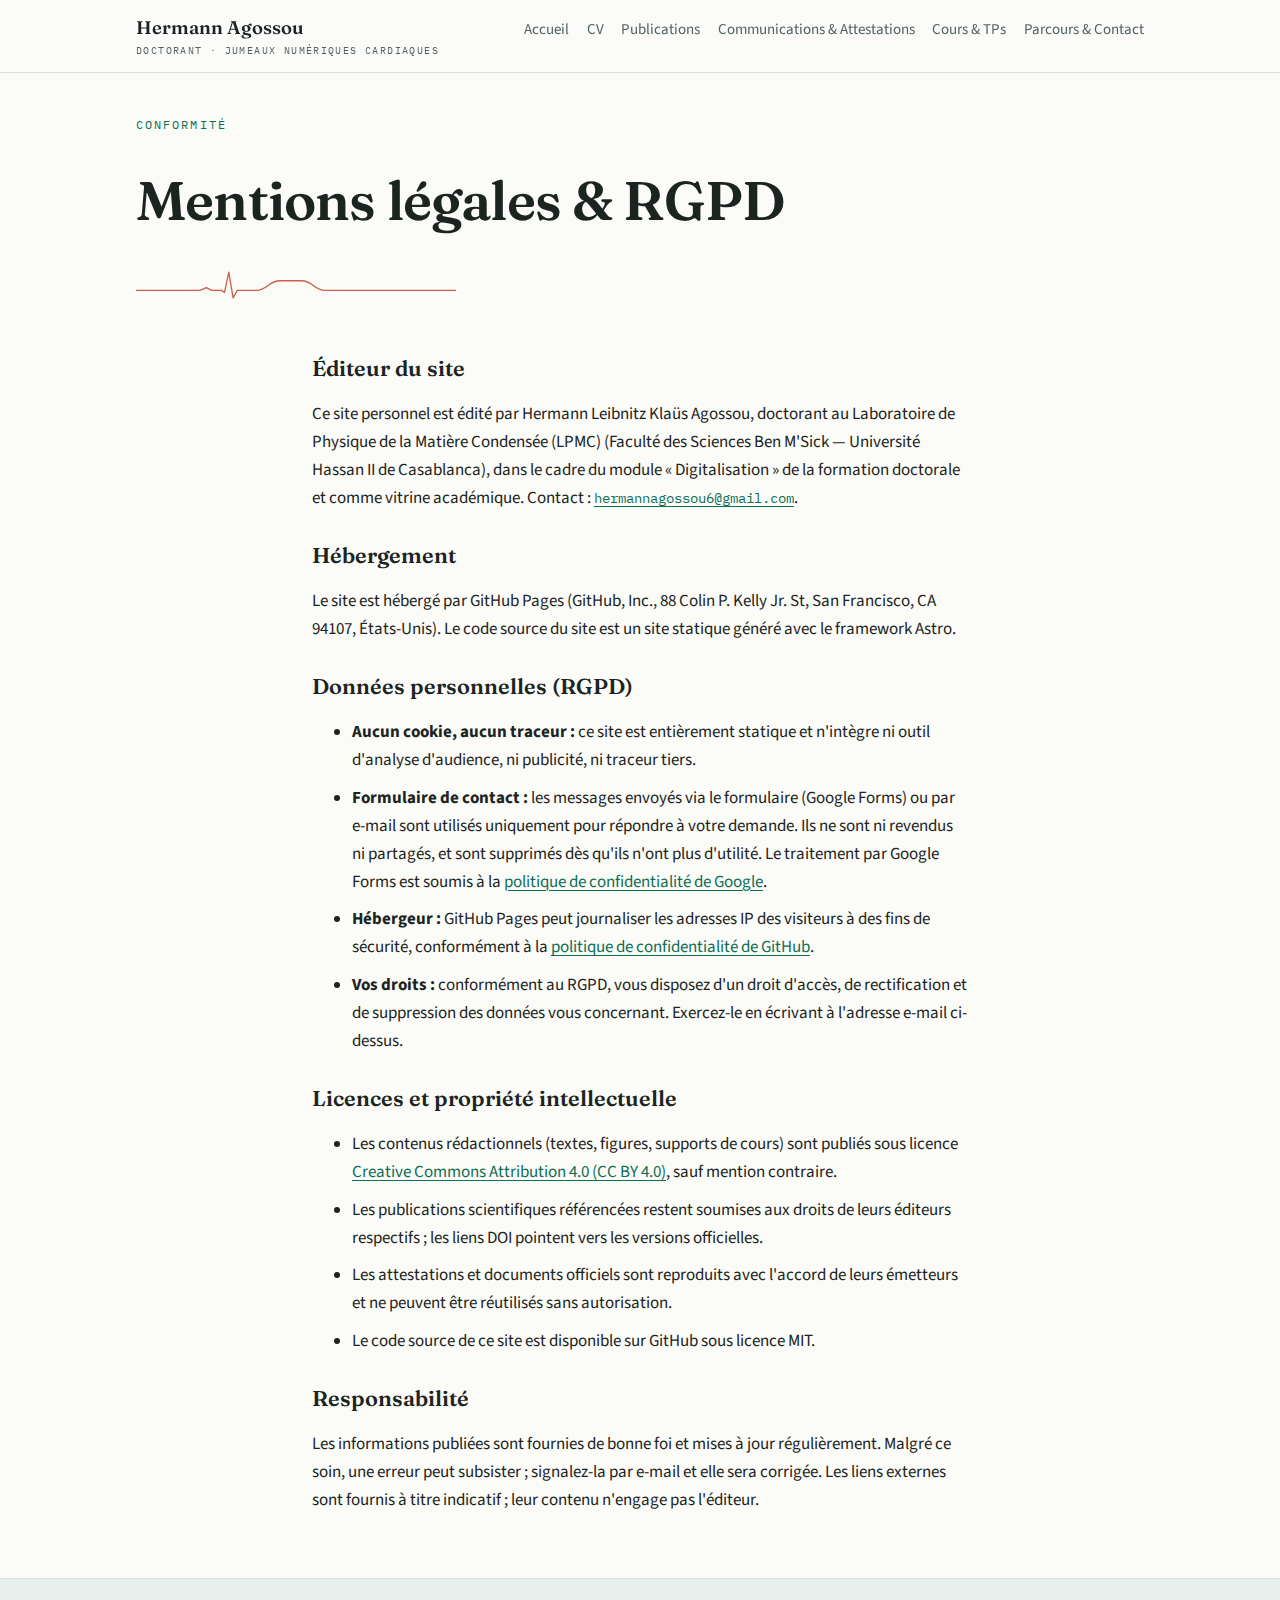
\includegraphics[width=0.96\linewidth]{assets/rgpd.png}}
  \caption{Mentions légales \& RGPD : éditeur, hébergement, gestion des données
    personnelles, licences.}
  \label{fig:rgpd}
\end{figure}

\clearpage

\section{Méthodologie}

La démarche suit les étapes du cahier des charges :

\begin{enumerate}[itemsep=2pt]
  \item \textbf{Planification} : arborescence figée en sept pages ; wireframe
    réalisé sous draw.io (\texttt{docs/wireframe.drawio} dans le dépôt).
  \item \textbf{Préparation des contenus} : CV mis à jour (publications,
    communications, intitulé de thèse) et compilé en PDF depuis LaTeX ;
    collection Zotero « COURSDIGIT » exportée en \texttt{.bib} ; attestations
    rassemblées et renommées proprement.
  \item \textbf{Construction du site} : projet Astro ; les contenus
    (publications, communications, attestations, cours, parcours) sont des
    fichiers de données typés, séparés de la mise en page, pour faciliter les
    mises à jour futures. La page Publications est générée automatiquement à
    partir de l'export Zotero.
  \item \textbf{Insertion et mise en forme} : CV intégré en visionneuse,
    attestations et supports en téléchargement direct, formulaire Google Forms
    intégré en iframe, mentions légales rédigées.
  \item \textbf{Contrôle qualité} : vérification TypeScript sans erreur, test
    mobile/desktop, vérification des liens et des téléchargements sur le site
    en ligne (toutes les pages répondent en HTTPS).
  \item \textbf{Publication} : déploiement automatique sur GitHub Pages à
    chaque mise à jour ; sous-domaine personnalisé
    \texttt{academic.hermann-agossou.com} (DNS Cloudflare, HTTPS).
\end{enumerate}

\section{Conformité éthique}

Le site n'utilise ni cookie ni traceur ; les messages du formulaire ne servent
qu'à répondre aux demandes. Les contenus rédactionnels sont publiés sous
licence CC~BY~4.0 ; les publications référencées pointent vers les versions
officielles de leurs éditeurs (liens DOI) ; les attestations sont reproduites
avec l'accord de leurs émetteurs. Les documents sources contenant des données
personnelles sensibles (pièce d'identité, date de naissance) sont exclus du
dépôt public, et la photo publiée a été nettoyée de ses métadonnées EXIF
(notamment les coordonnées GPS).

\section{Conclusion}

Toutes les exigences du cahier des charges sont couvertes, plusieurs étant
dépassées (7~pages au lieu de~6, 14~références au lieu de~10, 9~attestations au
lieu de~5, 5~supports au lieu de~3). Le site est en ligne sur \siteurl,
maintenable sur le long terme, et pourra évoluer tout au long du doctorat :
l'ajout d'une publication, d'une communication ou d'une attestation se résume à
éditer un fichier de données et à pousser la modification.

\end{document}
